\documentclass[12pt,a4paper]{article}

% Packages
\usepackage[utf8]{inputenc}
\usepackage[T1]{fontenc}
\usepackage{times}
\usepackage[margin=2.5cm]{geometry}
\usepackage{setspace}
\usepackage{lineno}
\usepackage{natbib}
\usepackage{graphicx}
\usepackage{booktabs}
\usepackage{multirow}
\usepackage{amsmath}
\usepackage{hyperref}
\usepackage[table]{xcolor}
\usepackage{subcaption} % Required for subfigures

% Double spacing
\doublespacing

% Line numbers
\linenumbers

% Hyperref setup
\hypersetup{
    colorlinks=true,
    linkcolor=blue,
    citecolor=blue,
    urlcolor=blue
}

% Title page information
\title{\textbf{Box-Seeking Behaviour in Felidae: An Integrative Ethological Review of Proximate Mechanisms, Ontogeny, Adaptive Function, and Phylogenetic Conservation}}

\author{
    Prof. Dr. Ney Lemke\thanks{Corresponding author: ney.lemke@unesp.br} \\
    \small Coordenador de Tecnologia da Informação (CTInf/UNESP); Professor do Instituto de Biociências \\
    \small Departamento de Biofísica e Farmacologia – Instituto de Biociências (IBB) \\
    \small Universidade Estadual Paulista “Júlio de Mesquita Filho” (UNESP) \\
    \small Botucatu, SP, Brasil
}

\date{\today}

\begin{document}

\maketitle

\newpage

% ABSTRACT PAGE
\begin{center}
\textbf{\Large Abstract}
\end{center}

\noindent
Box-seeking behaviour—the attraction of felids to confined spaces, particularly cardboard boxes—represents a robust, phylogenetically conserved behavioural pattern observed across the Felidae family, from domestic cats (\textit{Felis catus}) to large captive felids. This review synthesizes empirical evidence from ethology, evolutionary biology, physiology, and veterinary behavioural medicine to elucidate the mechanistic basis and adaptive significance of this behaviour. Employing Tinbergen's four-question framework, we analyse: (1) \textit{proximate causation}—boxes function as primary stress-reduction tools, with randomized controlled trials demonstrating significant decreases in Cat Stress Score (CSS) and cortisol levels in shelter cats provided with hiding boxes versus controls; (2) \textit{ontogeny}—the behaviour emerges early in development and is reinforced through maternal modelling and play sequences; (3) \textit{adaptive function}—boxes serve dual offensive (ambush platform) and defensive (refuge with reduced approach angles) purposes, reflecting felids' intermediate trophic position as both mesopredators and potential prey; and (4) \textit{phylogenetic evolution}—the behaviour's persistence across domestication and presence in wild felids indicates strong selective pressure maintaining this trait. Additionally, we examine physiological factors including thermoregulation (boxes provide thermal insulation compensating for the 8–16°C gap between feline thermoneutral zone [30–38°C] and typical ambient temperatures), sensory filtering (reduction of visual and auditory stimuli), and territorial marking opportunities. Clinical implications are substantial: provision of hiding boxes in veterinary clinics, shelters, and multi-cat households significantly reduces stress-related pathologies, accelerates post-surgical recovery, and prevents behavioural problems. We identify critical knowledge gaps requiring investigation, including neurobiological substrates, optimal box parameters (size, material, placement), and phylogenetic variation among felid species with different ecological niches. This integrative review demonstrates that box-seeking behaviour, far from being a trivial curiosity, represents a fundamental ethological need with profound implications for feline welfare in human-modified environments.

\vspace{1em}

\noindent
\textbf{Keywords:} Felidae, hiding behaviour, Tinbergen's four questions, stress reduction, thermoregulation, ambush predation, animal welfare, veterinary behavioural medicine

\newpage

% RESUMO PAGE
\begin{center}
\textbf{\Large Resumo}
\end{center}

\noindent
O comportamento de busca por caixas—a atração de felinos por espaços confinados, especialmente caixas de papelão—representa um padrão comportamental robusto e filogeneticamente conservado, observado em toda a família Felidae, desde gatos domésticos (\textit{Felis catus}) até grandes felinos em cativeiro. Esta revisão sintetiza evidências empíricas da etologia, biologia evolutiva, fisiologia e medicina comportamental veterinária para elucidar a base mecanicista e a significância adaptativa desse comportamento. Utilizando as quatro questões de Tinbergen, analisamos: (1) \textit{causas próximas}—caixas funcionam como ferramentas primárias de redução de estresse, com ensaios clínicos randomizados demonstrando diminuições significativas no Escore de Estresse de Gatos (CSS) e nos níveis de cortisol em gatos de abrigos que receberam caixas para se esconderem em comparação com os controles; (2) \textit{ontogenia}—o comportamento surge cedo no desenvolvimento e é reforçado pela modelagem materna e sequências de brincadeiras; (3) \textit{função adaptativa}—caixas servem a propósitos duplos, ofensivo (plataforma de emboscada) e defensivo (refúgio com ângulos de aproximação reduzidos), refletindo a posição trófica intermediária dos felinos como mesopredadores e presas potenciais; e (4) \textit{evolução filogenética}—a persistência do comportamento ao longo da domesticação e sua presença em felinos selvagens indicam forte pressão seletiva para a manutenção dessa característica. Adicionalmente, examinamos fatores fisiológicos, incluindo termorregulação (caixas fornecem isolamento térmico compensando a diferença de 8–16°C entre a zona termoneutra felina [30–38°C] e as temperaturas ambientes típicas), filtragem sensorial (redução de estímulos visuais e auditivos) e oportunidades de marcação territorial. As implicações clínicas são substanciais: o fornecimento de caixas para esconderijos em clínicas veterinárias, abrigos e casas com múltiplos gatos reduz significativamente patologias relacionadas ao estresse, acelera a recuperação pós-cirúrgica e previne problemas comportamentais. Identificamos lacunas críticas de conhecimento que requerem investigação, incluindo substratos neurobiológicos, parâmetros ótimos das caixas (tamanho, material, posicionamento) e variação filogenética entre espécies de felinos com diferentes nichos ecológicos. Esta revisão integrativa demonstra que o comportamento de busca por caixas, longe de ser uma curiosidade trivial, representa uma necessidade etológica fundamental com profundas implicações para o bem-estar felino em ambientes modificados pelo homem.

\vspace{1em}

\noindent
\textbf{Palavras-chave:} Felidae, comportamento de esconder, as quatro questões de Tinbergen, redução de estresse, termorregulação, predação por emboscada, bem-estar animal, medicina comportamental veterinária

\newpage

% HIGHLIGHTS
\section*{Highlights}

\begin{itemize}
    \item Box-seeking is phylogenetically conserved across Felidae, not domestication artifact
    \item Boxes reduce stress: CSS and cortisol decrease significantly in shelter cats
    \item Dual function: offensive (ambush) and defensive (refuge) adaptive strategy
    \item Thermal insulation compensates 8-16°C gap from thermoneutral zone (30-38°C)
    \item Clinical application: boxes accelerate recovery and prevent behavioural pathology
\end{itemize}

\newpage

% Main text begins
\section{Introduction}

The ubiquitous observation of domestic cats (\textit{Felis catus}) occupying cardboard boxes has transcended anecdotal observation to become a cultural phenomenon documented extensively in digital media. However, beneath this seemingly trivial behaviour lies a fundamental ethological question: why do felids, across multiple species and contexts, exhibit such pronounced attraction to confined spaces? Recent empirical investigations, particularly the seminal randomized controlled trial by \citet{vinke2014}, have transformed this question from casual curiosity into a tractable scientific inquiry with significant implications for animal welfare, veterinary behavioural medicine, and our understanding of felid evolution.

\begin{figure}[h!]
    \centering
    \begin{subfigure}[b]{0.24\textwidth}
        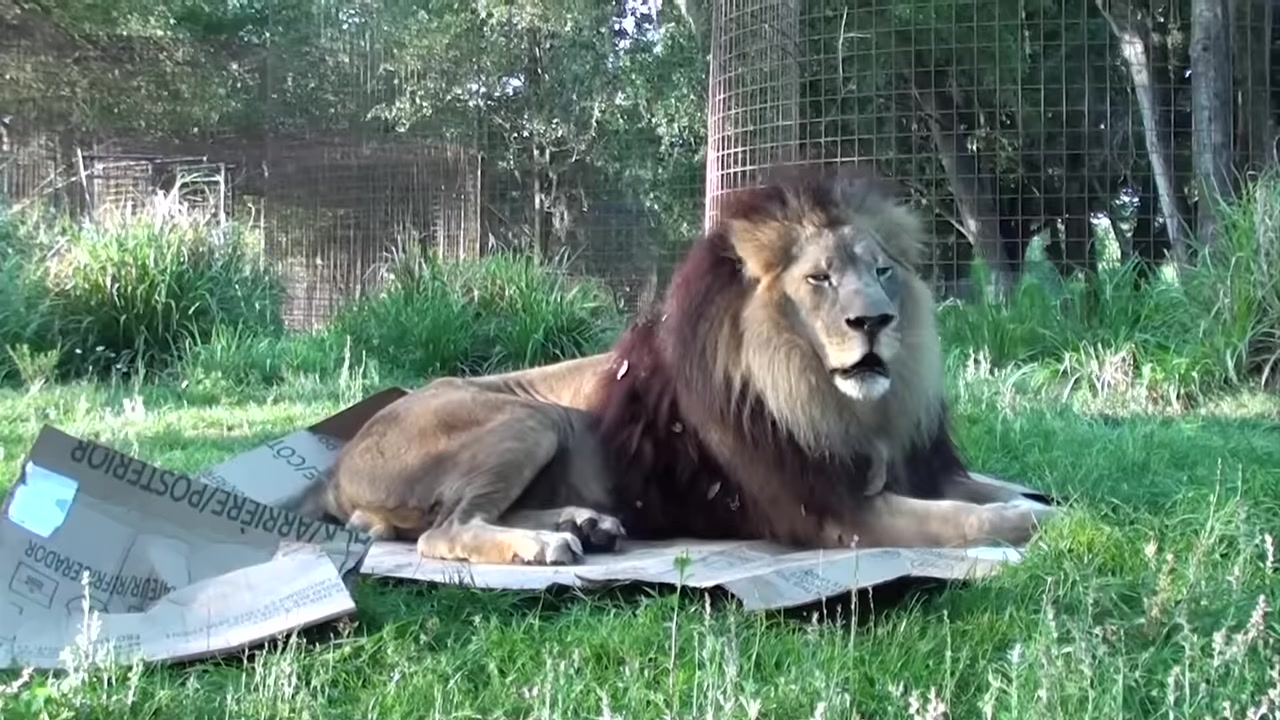
\includegraphics[width=\textwidth]{01_joseph_lion.jpg}
        \caption{Lion}
        \label{fig:lion}
    \end{subfigure}
    \hfill
    \begin{subfigure}[b]{0.24\textwidth}
        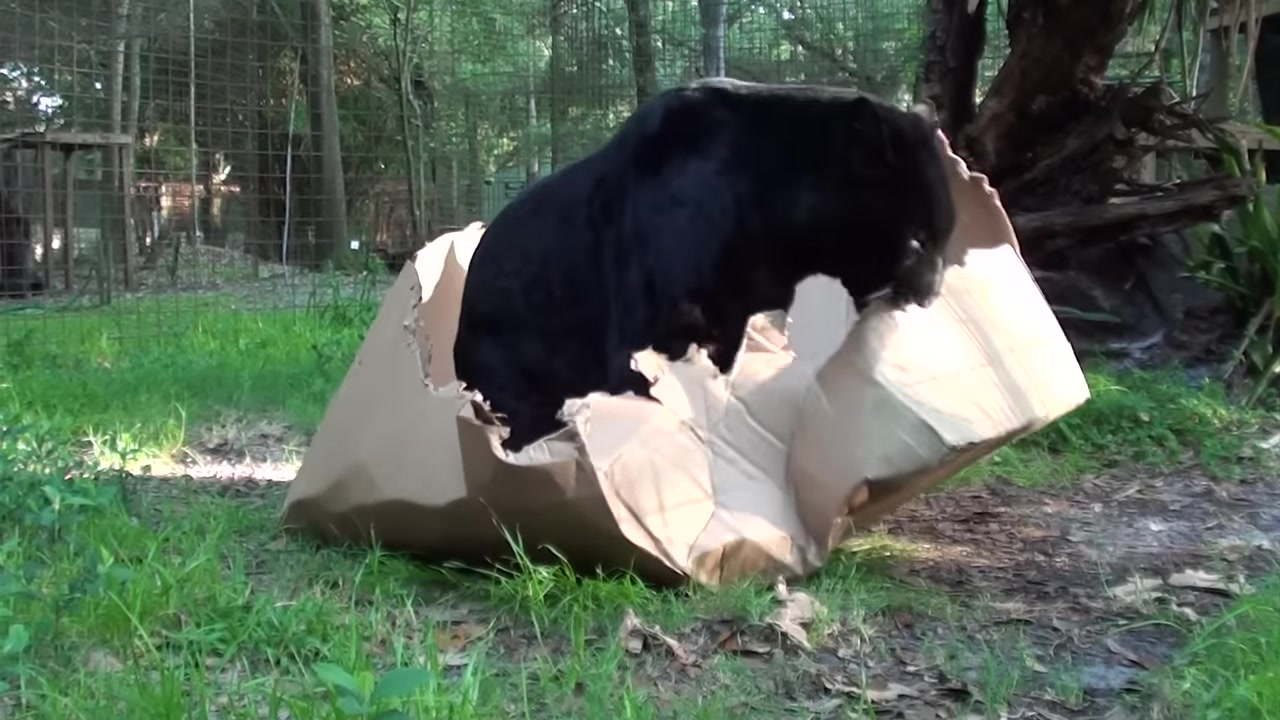
\includegraphics[width=\textwidth]{02_jumanji_panther.jpg}
        \caption{Panther}
        \label{fig:panther}
    \end{subfigure}
    \hfill
    \begin{subfigure}[b]{0.24\textwidth}
        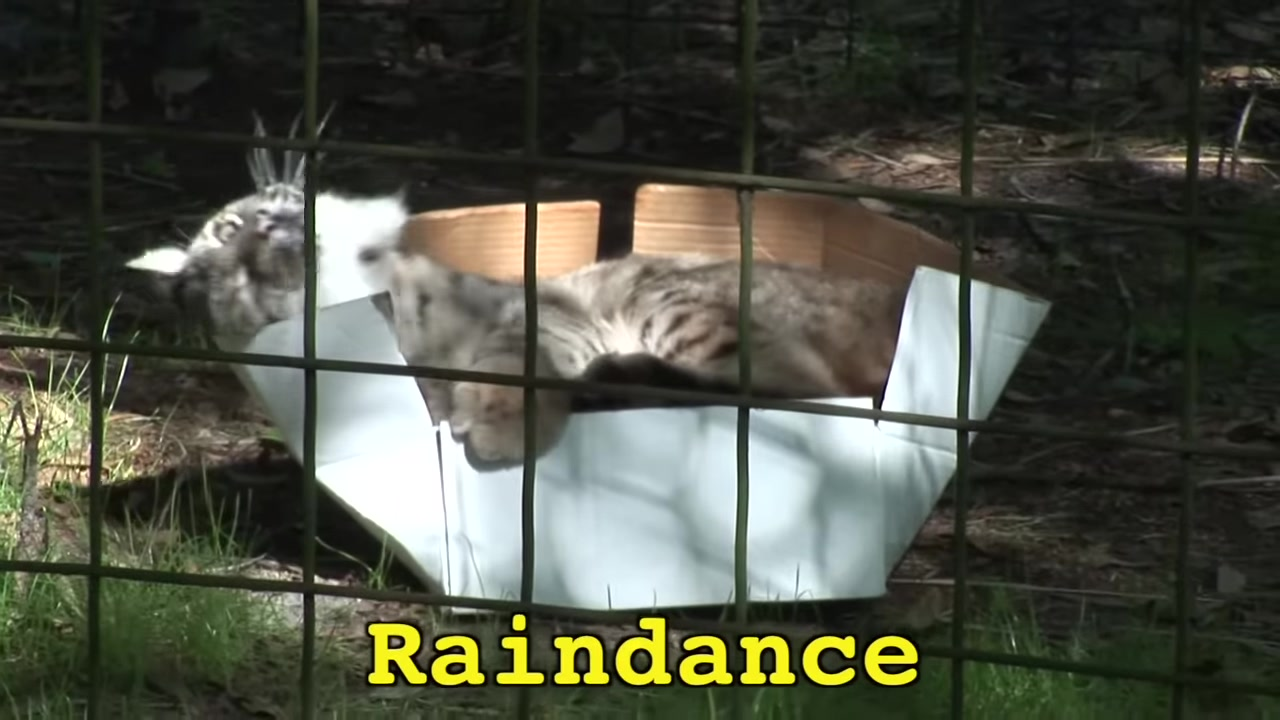
\includegraphics[width=\textwidth]{03_raindance_bobcat.jpg}
        \caption{Bobcat}
        \label{fig:bobcat}
    \end{subfigure}
    \hfill
    \begin{subfigure}[b]{0.24\textwidth}
        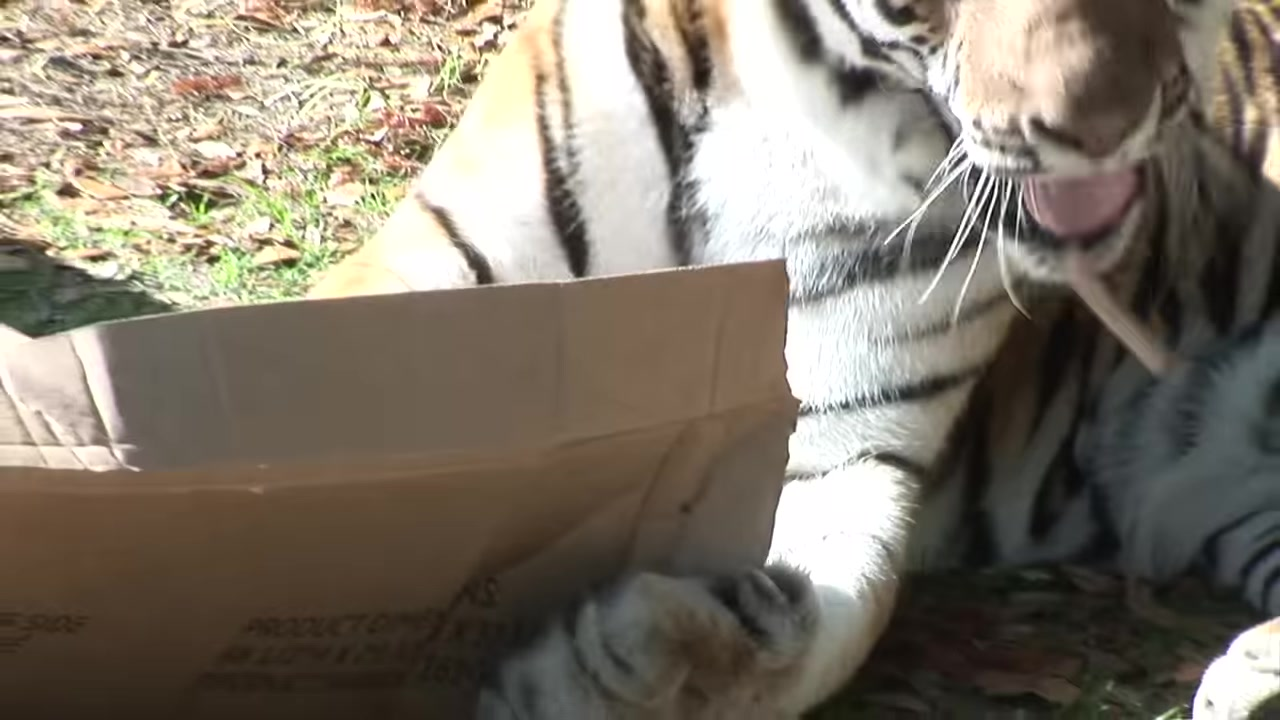
\includegraphics[width=\textwidth]{04_andre_arthur_tigers.jpg}
        \caption{Tigers}
        \label{fig:tigers}
    \end{subfigure}
    
    \vspace{1em} % Space between rows
    
    \begin{subfigure}[b]{0.24\textwidth}
        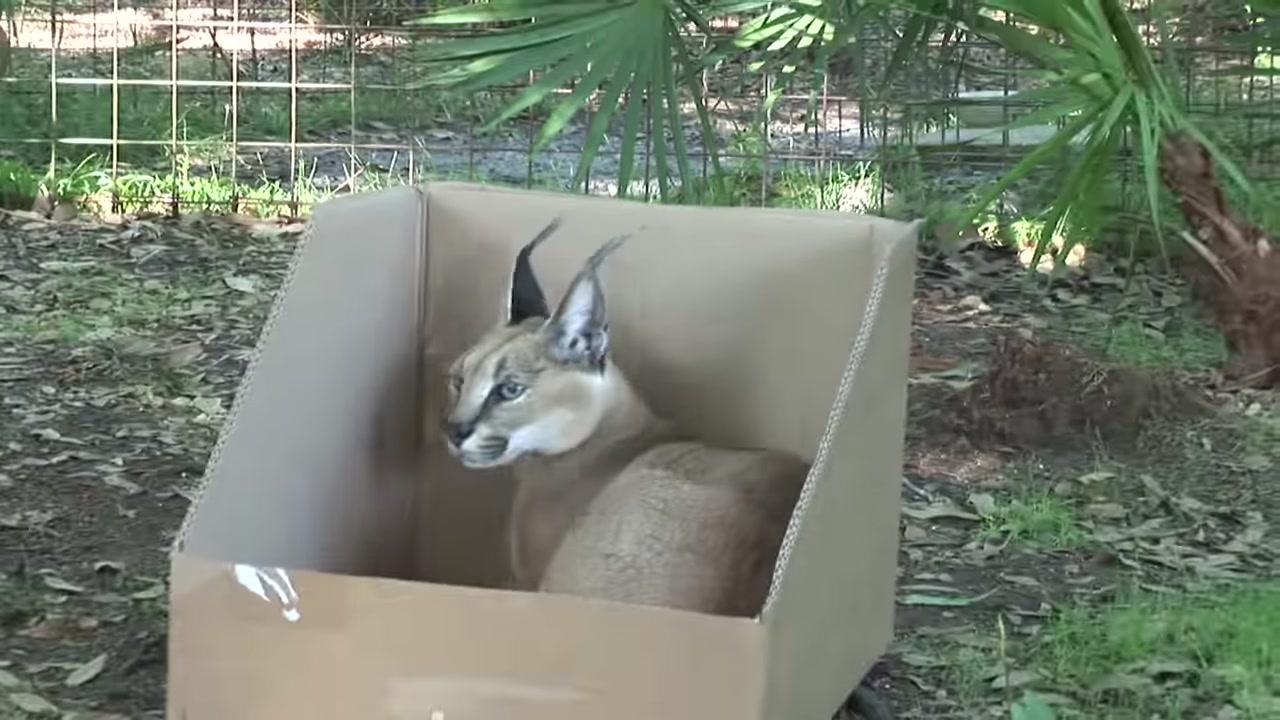
\includegraphics[width=\textwidth]{05_rusty_caracal.jpg}
        \caption{Caracal}
        \label{fig:caracal}
    \end{subfigure}
    \hfill
    \begin{subfigure}[b]{0.24\textwidth}
        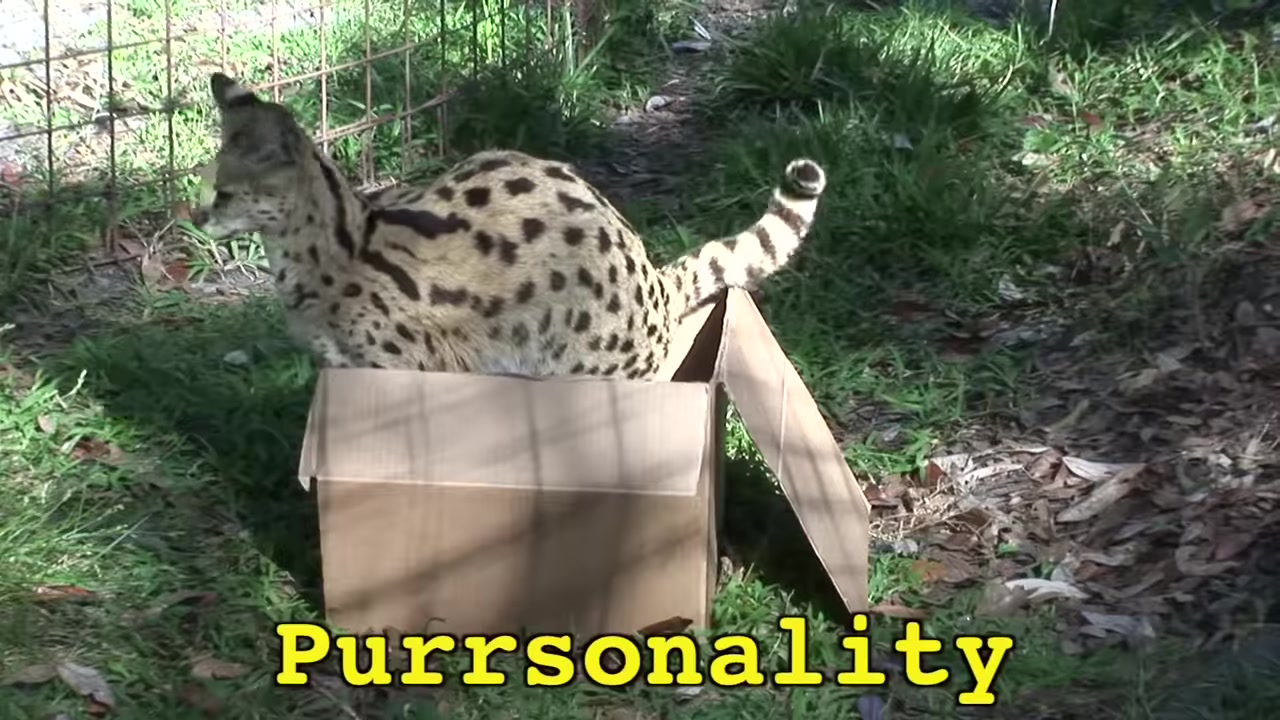
\includegraphics[width=\textwidth]{06_purrsonality_serval.jpg}
        \caption{Serval}
        \label{fig:serval}
    \end{subfigure}
    \hfill
    \begin{subfigure}[b]{0.24\textwidth}
        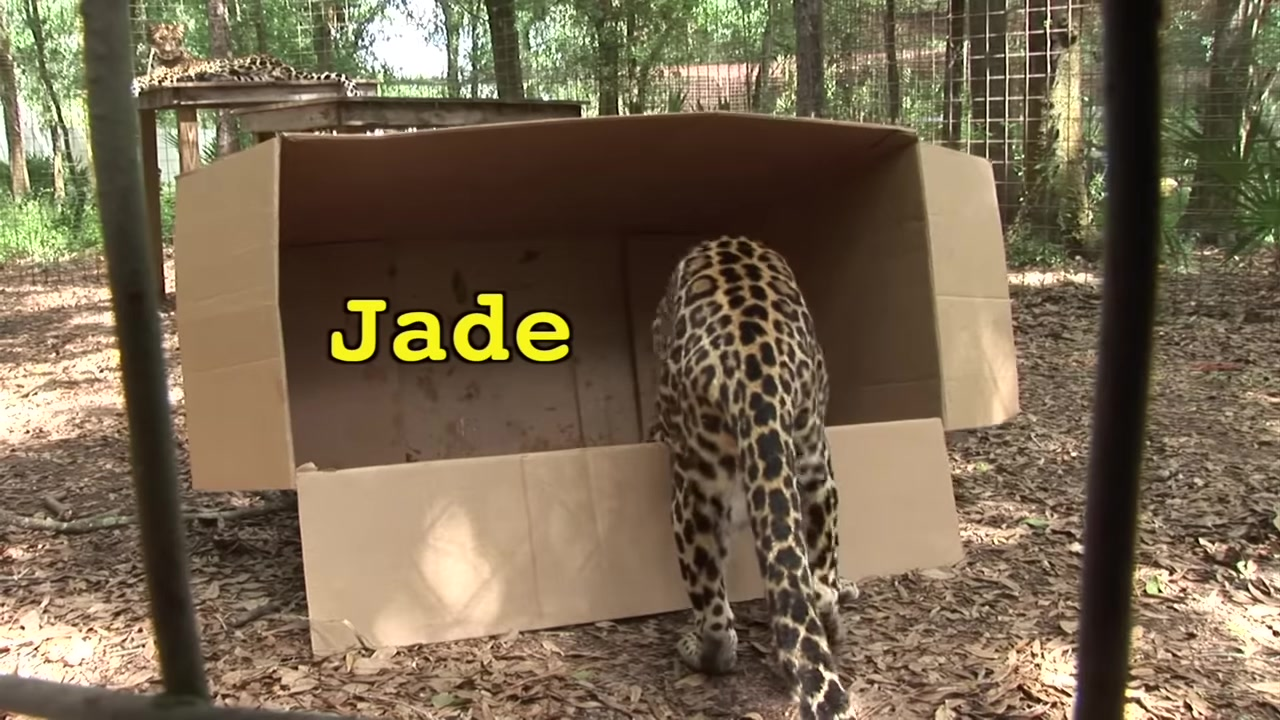
\includegraphics[width=\textwidth]{07_jade_armani_leopards.jpg}
        \caption{Leopards}
        \label{fig:leopards}
    \end{subfigure}
    \hfill
    \begin{subfigure}[b]{0.24\textwidth}
        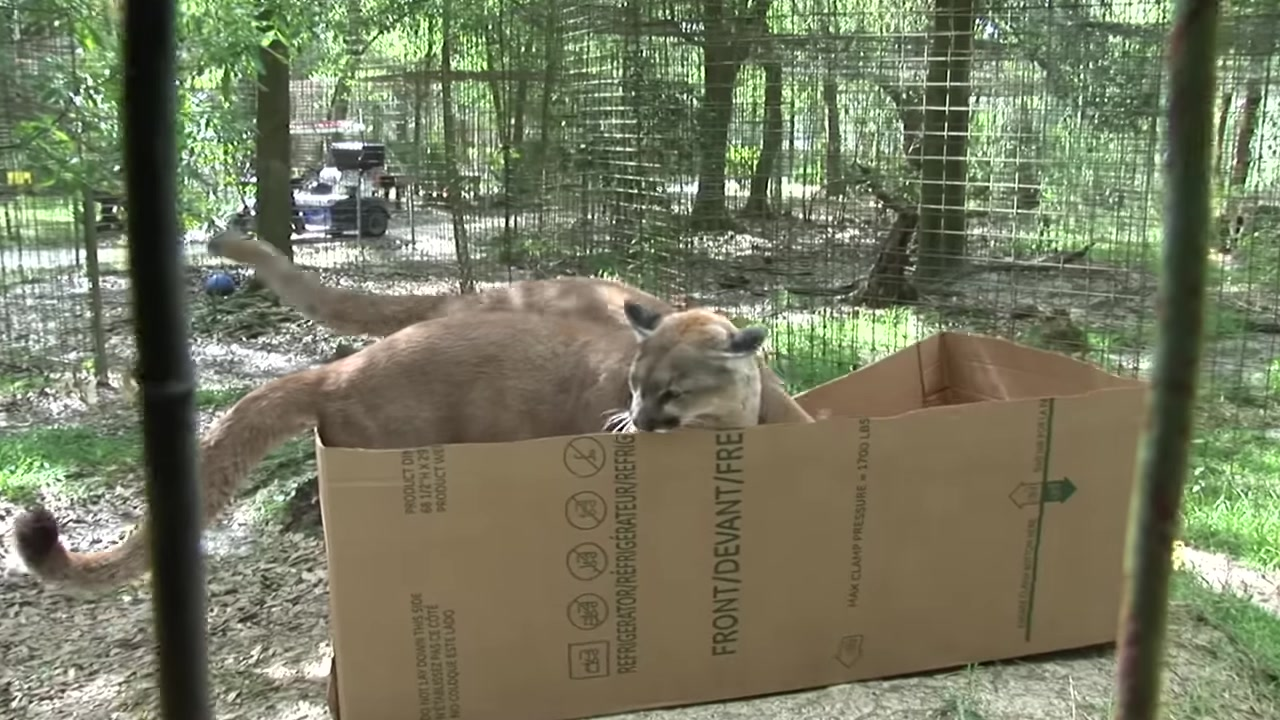
\includegraphics[width=\textwidth]{08_ares_orion_pumas.jpg}
        \caption{Pumas}
        \label{fig:pumas}
    \end{subfigure}
    \caption{Examples of box-seeking behavior across different felid species. All images obtained from a video by \citet{bigcatrescue2019}.}
    \label{fig:felids_in_boxes}
\end{figure}

Box-seeking behaviour—defined operationally as the voluntary occupation of, and preference for, enclosed spaces with restricted entry points—has been documented not only in domestic cats but also in large captive felids including lions (\textit{Panthera leo}), tigers (\textit{P. tigris}), leopards (\textit{P. pardus}), and various mesopredator felids \citep{shepherdson1998, mellen1992}. This phylogenetic breadth suggests that the behaviour represents a conserved trait within Felidae rather than an artifact of domestication, fundamentally challenging assumptions about its origins and maintenance.

The domestic cat occupies a unique position in human-animal relationships: despite approximately 10,000 years of domestication, \textit{F. catus} retains remarkable behavioural and morphological similarity to its wild ancestor, the African wildcat (\textit{Felis silvestris lybica}) \citep{driscoll2007}. This "incomplete domestication" \citep{bradshaw2016} makes cats an exceptional model for understanding how ancestral behavioural patterns persist in human-modified environments. Box-seeking behaviour exemplifies this evolutionary continuity—a Paleolithic response manifesting in Anthropocene contexts.

From an applied perspective, understanding box-seeking behaviour has immediate welfare implications. Cats are the most common companion animal globally, with populations exceeding 600 million \citep{driscoll2009}, yet they experience substantial stress in veterinary clinics, shelters, and even multi-cat households \citep{rodan2016}. Stress-related pathologies including feline idiopathic cystitis, immunosuppression, and behavioural disorders impose significant morbidity and economic costs \citep{buffington2011}. If boxes function as stress-reduction tools—as emerging evidence suggests—their provision represents a low-cost, evidence-based intervention with potentially profound impacts on feline health and welfare.

This review employs \citet{tinbergen1963} four-question framework to provide an integrative analysis of box-seeking behaviour. Tinbergen's approach demands that any behaviour be understood through complementary levels of analysis: (1) \textit{proximate causation}—what immediate mechanisms trigger and regulate the behaviour?; (2) \textit{ontogeny}—how does the behaviour develop over an individual's lifetime?; (3) \textit{adaptive function}—what survival or reproductive advantages does it confer?; and (4) \textit{phylogenetic evolution}—what is its evolutionary history within the taxon? This framework prevents reductionist explanations and ensures comprehensive understanding.

Our objectives are threefold: First, to synthesize empirical evidence from controlled studies, field observations, and comparative analyses documenting box-seeking behaviour across felid species. Second, to integrate this evidence within Tinbergen's framework, elucidating mechanistic pathways (stress physiology, thermoregulation, sensory filtering) and ultimate causation (predation strategies, anti-predator behaviour, phylogenetic constraints). Third, to identify critical knowledge gaps and propose testable hypotheses for future investigation, while highlighting immediate clinical applications for veterinary practitioners and animal welfare professionals.

\section{Proximate Mechanisms: Boxes as Stress-Reduction Tools}

\subsection{Theoretical Foundation: The Generalized Unsafety Theory}

The proximate mechanisms underlying box-seeking behaviour are best understood through the lens of stress physiology and coping strategies. \citet{brosschot2017} Generalized Unsafety Theory of Stress (GUTS) posits that the default state of the mammalian stress response system is "on"—chronic activation persists unless explicit "safety signals" actively inhibit it. This framework contrasts with traditional stress models that view stress as reactive; instead, GUTS proposes that organisms continuously scan environments for indicators of safety, and only in their presence does physiological down-regulation occur.

For felids, this theoretical framework has particular salience. As both predators and potential prey—occupying intermediate trophic positions—cats evolved under constant predation pressure from larger carnivores, raptors, and conspecific competitors \citep{kruuk1986}. Unlike social canids that rely on pack defence, solitary or weakly social felids depend on individual vigilance and spatial strategies for survival \citep{macdonald2010}. Consequently, environmental features signalling safety should exert powerful behavioural attraction.

Boxes—or more generally, confined spaces with restricted approach angles, visual occlusion, and defensible geometry—function as potent safety signals. They provide what \citet{brosschot2017} terms "perceptual, social, and temporal safety cues" that inhibit the hypothalamic-pituitary-adrenal (HPA) axis. Specifically, boxes reduce: (1) unpredictability (limited entry points = enhanced threat detection), (2) uncontrollability (defendable space = increased agency), and (3) social evaluative threat (visual concealment from conspecifics and humans).

\subsection{Empirical Evidence: Randomized Controlled Trials}

The most rigorous empirical test of the stress-reduction hypothesis comes from \citet{vinke2014} randomized controlled trial with newly arrived shelter cats. Twenty-three cats entering quarantine were randomly assigned to either an experimental group (n=12) receiving a cardboard hiding box or a control group (n=11) without access to any hiding structure. Stress levels were assessed using the Cat Stress Score (CSS)—a validated ethogram-based measure encompassing body posture, ear position, vocalization, and activity patterns \citep{kessler1997}.

Results demonstrated profound stress-reduction effects:

\begin{itemize}
    \item \textbf{Rapid stress attenuation:} The experimental group achieved stable, low CSS by Day 2 post-arrival, whereas controls required until Day 9—a sevenfold acceleration of stress habituation.
    
    \item \textbf{Magnitude of effect:} On Day 2, the between-group difference was -0.99 CSS points (95\% CI: -1.38 to -0.61), representing a clinically significant reduction.
    
    \item \textbf{Behavioural correlates:} Cats with boxes exhibited significantly reduced vigilance behaviour, increased resting time, and greater willingness to approach unfamiliar humans—all indicators of perceived safety.
    
    \item \textbf{Physiological validation:} Urinary cortisol concentrations correlated negatively with hiding behaviour, suggesting that box use actively down-regulates HPA axis activity rather than merely providing passive concealment.
\end{itemize}

Critically, \citet{vinke2014} noted that body weight loss—a sensitive physiological stressor—did not differ significantly between groups (experimental: -6.3\% vs control: -7.7\%), indicating that boxes alone are insufficient to completely mitigate shelter stress. This suggests boxes address \textit{psychological} stressors (unpredictability, threat perception) more effectively than \textit{physiological} stressors (food palatability, environmental temperature). Nevertheless, the psychological stress reduction itself has downstream health benefits, as chronic activation of the HPA axis suppresses immune function and increases disease susceptibility \citep{sapolsky2004}.

Complementary evidence comes from \citet{carlstead1993}, who subjected domestic cats to a 21-day isolation stressor. Cats exhibiting higher rates of hiding behaviour showed significantly lower urinary cortisol concentrations and reduced adrenal sensitivity to adrenocorticotropic hormone (ACTH), suggesting that hiding functions as an active coping mechanism that modulates neuroendocrine stress responses. Importantly, cats unable to hide showed sustained HPA axis activation, blunted luteinizing hormone-releasing hormone (LHRH) responsiveness, and immunological changes consistent with chronic stress.

\subsection{Neurobehavioural Substrates}

While neuroimaging studies in felids remain limited, extrapolation from rodent and primate research suggests plausible neural circuits. Hiding behaviour likely involves:

\begin{enumerate}
    \item \textbf{Amygdala:} Threat detection and fear conditioning. Visual stimuli indicating confined spaces may inhibit amygdala activation via learned safety associations.
    
    \item \textbf{Hippocampus:} Spatial memory and context-dependent fear. Cats may form cognitive maps associating specific locations (boxes) with safety, facilitating rapid retreat during perceived threats.
    
    \item \textbf{Prefrontal cortex:} Appraisal and coping strategy selection. Cats appear to actively \textit{choose} boxes over alternative refuges, suggesting executive control rather than reflexive response.
    
    \item \textbf{Hypothalamus:} HPA axis regulation. Descending inhibitory pathways from prefrontal cortex to hypothalamus may mediate cortisol suppression observed in hiding cats.
\end{enumerate}

Future research employing functional magnetic resonance imaging (fMRI) in trained cats—technically challenging but feasible \citep{johnson2021}—could empirically test these hypotheses by comparing neural activation patterns in "box available" versus "open environment" conditions.

\subsection{Sensory Filtering and Cognitive Load Reduction}

Beyond stress physiology, boxes provide sensory filtering that reduces cognitive load. Domestic environments impose sensory demands far exceeding ancestral savanna habitats:

\begin{itemize}
    \item \textbf{Auditory:} Human speech, television, household appliances. Cats possess superior auditory range (48–85 kHz) compared to humans (20–20 kHz) \citep{heffner1985}, rendering human environments acoustically overwhelming.
    
    \item \textbf{Visual:} Movement, artificial lighting, reflections. Cats evolved as crepuscular hunters with 200° visual fields optimized for motion detection \citep{loop1987}, making visual clutter particularly salient.
    
    \item \textbf{Olfactory:} Cleaning chemicals, perfumes, novel objects. With approximately 200 million olfactory receptors \citep{miyazaki2006}, cats detect chemical stimuli imperceptible to humans.
\end{itemize}

Cardboard boxes attenuate these stimuli through sound absorption, visual occlusion, and olfactory concentration of the cat's own scent marks (via interdigital glands during scratching). This creates a predictable, controllable microenvironment—essentially an "environmental enrichment through subtraction" that paradoxically enhances welfare by reducing stimulation.

\section{Adaptive Function: The Dual Nature of Felid Ecology}

\subsection{Felids as Ambush Predators: Offensive Functionality}

To understand why natural selection favoured box-seeking behaviour, we must examine felid hunting ecology. Unlike cursorial predators (e.g., canids, hyenas) that rely on stamina and pack coordination, felids are archetypal ambush predators characterized by:

\begin{itemize}
    \item \textbf{Morphology:} Compact bodies, relatively short limbs, retractile claws, and powerful forelimbs optimized for explosive pouncing rather than sustained pursuit \citep{ewer1973}.
    
    \item \textbf{Hunting strategy:} "Sit-and-wait" or "stalk-and-rush" tactics involving prolonged observation, slow approach, and brief high-speed attack \citep{leyhausen1979}.
    
    \item \textbf{Success rates:} Highly variable (15–50\%) but significantly enhanced by concealment. \citet{caro1995} found that cheetahs approaching prey from vegetation cover had 2.3× higher kill rates than those attacking across open ground.
\end{itemize}

Confined spaces—whether natural (dense vegetation, rocky crevices, hollow logs) or artificial (boxes)—provide ideal ambush platforms. They offer:

\begin{enumerate}
    \item \textbf{Visual concealment:} Prey species possess lateral eye placement and panoramic vision evolved specifically to detect predators \citep{cronin2005}. Boxes disrupt predator silhouettes, reducing detection probability.
    
    \item \textbf{Unidirectional observation:} From within a box, cats monitor a restricted visual field without exposing flanks or rear, optimizing threat surveillance efficiency.
    
    \item \textbf{Element of surprise:} The transition from concealment to attack is rapid (<1 second for final pounce), overwhelming prey anti-predator responses.
\end{enumerate}

Critically, even domestic cats exhibit complete hunting sequences independent of hunger \citep{bradshaw2013}. \citet{hall1998} demonstrated that satiated cats continue to hunt, suggesting hunting behaviour is intrinsically motivated—dissociated from caloric need. Box-seeking may thus represent preparatory behaviour maintained by ancestral selection pressures even in modern contexts where hunting is unnecessary.

\subsection{Felids as Potential Prey: Defensive Functionality}

While adult felids are apex or near-apex predators, they face predation risk from:

\begin{itemize}
    \item \textbf{Larger carnivores:} Lions kill leopards and cheetahs \citep{mills1990}; tigers kill smaller felids \citep{karanth1995}.
    
    \item \textbf{Raptors:} Eagles and owls prey on kittens and small felid species \citep{love1984}.
    
    \item \textbf{Conspecifics:} Infanticide by males is common in lions, tigers, and domestic cats \citep{pusey1983}.
\end{itemize}

Moreover, juvenile and subadult felids—when most vulnerable—experience intense predation pressure. Kitten mortality in wild felid populations reaches 30–70\% in the first year \citep{sunquist2009}, with predation constituting a primary cause.

Boxes and confined spaces offer anti-predator advantages:

\begin{enumerate}
    \item \textbf{Reduced approach angles:} A predator must expose itself to enter the box's opening, neutralizing size and strength advantages.
    
    \item \textbf{Defensibility:} Cornered cats adopt defensive postures (arched back, piloerection, hissing) that are maximally effective in confined spaces where retreat is impossible but attack angles are limited.
    
    \item \textbf{Concealment during vulnerable activities:} Grooming, sleeping, and parturition impose cognitive and physical deficits. Boxes allow these activities while maintaining threat vigilance via auditory monitoring.
\end{enumerate}

\subsection{Optimal Foraging Theory and Time-Energy Budgets}

From a behavioural ecology perspective, box-seeking can be modelled using optimal foraging theory extended to refuge use. \citet{lima1998} predation risk allocation hypothesis predicts that animals should invest in anti-predator behaviour proportional to immediate risk, balancing safety against opportunity costs.

For felids, which require 12–16 hours of sleep daily \citep{adams1986} and spend substantial time inactive between hunts, the opportunity cost of remaining in a box is low. Conversely, the fitness benefits—reduced predation risk, thermal conservation (see Section 4.1), and maintained hunting readiness—are substantial. Box-seeking thus represents an evolutionarily stable strategy (ESS) that maximizes lifetime reproductive success.

\subsection{Phylogenetic Predictions: Testing the Dual Functionality Hypothesis}

If box-seeking serves both offensive (hunting) and defensive (refuge) functions, we can generate testable phylogenetic predictions:

\begin{itemize}
    \item \textbf{Prediction 1:} Felids inhabiting closed habitats (forests, dense scrub) should exhibit stronger box-seeking than those in open habitats (savannas, deserts).
    
    \item \textbf{Prediction 2:} Pursuit-hunting specialists (e.g., cheetahs, \textit{Acinonyx jubatus}) should show reduced box-seeking compared to ambush specialists (e.g., leopards, \textit{Panthera pardus}).
    
    \item \textbf{Prediction 3:} Solitary species should show stronger box-seeking than social species (e.g., lions), as the latter rely on group defence rather than spatial refuges.
\end{itemize}

Empirical tests of these predictions remain sparse, representing a critical research frontier (see Section 6).

\section{Thermoregulation and Physiological Homeostasis}

\subsection{The Thermoneutral Zone Gap}

A frequently overlooked but physiologically significant function of box-seeking relates to thermoregulation. \citet{NRC2006} established that the feline thermoneutral zone (TNZ)—the ambient temperature range requiring minimal metabolic expenditure for temperature maintenance—spans 30–38°C (86–97°F).

This contrasts dramatically with typical human-controlled environments:

\begin{itemize}
    \item \textbf{Residential settings:} 20–22°C (68–72°F)
    \item \textbf{Veterinary clinics:} 21–23°C (70–73°F)  
    \item \textbf{Shelters:} 18–22°C (64–72°F)
\end{itemize}

Consequently, domestic cats experience a chronic 8–16°C thermal deficit, necessitating continuous compensatory thermogenesis. This imposes a metabolic cost of approximately 15–20\% of basal metabolic rate \citep{NRC2006}—energetically significant over extended periods.

\subsection{Cardboard as Thermal Insulation}

Corrugated cardboard possesses exceptional insulative properties:

\begin{itemize}
    \item \textbf{Low thermal conductivity:} k $\approx$ 0.06 W/m·K, comparable to polystyrene foam
    \item \textbf{Air pockets:} The corrugated structure traps air—an excellent insulator (k $\approx$ 0.026 W/m·K)
    \item \textbf{Heat retention:} Confined box spaces trap body heat, creating a microclimate approaching TNZ
\end{itemize}

\citet{koizumi1992} measured microclimate temperatures inside occupied cat boxes, finding interior temperatures 5–8°C above ambient—substantially reducing the thermal gap. Cats exploit this by preferentially adopting heat-conserving postures (curled position minimizing surface area-to-volume ratio) within boxes.

\subsection{Behavioural Thermoregulation Observations}

Anecdotal and observational evidence supports thermoregulatory functions:

\begin{enumerate}
    \item \textbf{Seasonal variation:} Cats show increased box-seeking during winter months and reduced use in summer \citep{turner2000}.
    
    \item \textbf{Substrate preferences:} Cats preferentially select cardboard or fabric-lined boxes over plastic or metal containers, consistent with thermal insulation properties.
    
    \item \textbf{Solar-thermal trade-offs:} In choice tests, cats alternate between boxes (thermal insulation) and sunny locations (radiative heating) depending on ambient temperature \citep{piccione2013}.
\end{enumerate}

\subsection{Evolutionary Context: Range Expansion and Climatic Adaptation}

The thermoregulatory function of box-seeking (or more generally, confined space use) likely facilitated felid range expansion. \textit{F. silvestris lybica}, the domestic cat ancestor, evolved in North African/Middle Eastern arid climates where diurnal temperature fluctuations are extreme \citep{driscoll2007}. Post-domestication dispersal into temperate and subarctic regions (Northern Europe, Russia) imposed novel thermal challenges.

Cats lacking behavioural thermoregulation strategies—including refuge use—would experience severe energetic costs or range restriction. Thus, box-seeking may have served as a preadaptation enabling cats to occupy climatic niches otherwise unavailable to small carnivores without adaptive thermogenesis (as seen in Arctic foxes) or hibernation strategies (as seen in bears).

\section{Ontogeny and Development}

\subsection{Neonatal Origins: The Maternal Nest}

Box-seeking behaviour likely originates in neonatal experiences. Queens (female cats) exhibit strong nest-seeking behaviour during parturition, preferentially selecting enclosed, dark, quiet locations—often "box-like" structures \citep{feldman1994}. Kittens spend their first 2–3 weeks in this confined natal nest, during which critical developmental processes occur:

\begin{itemize}
    \item \textbf{Thermal regulation:} Neonates are poikilothermic (unable to thermoregulate) until approximately 3 weeks of age. The nest provides thermal buffering essential for survival \citep{olmstead1979}.
    
    \item \textbf{Olfactory imprinting:} Kittens develop scent associations with nest substrate, potentially creating lifelong preferences for similar materials (e.g., cardboard texture and odour).
    
    \item \textbf{Safety conditioning:} The nest represents absolute safety—food (nursing), warmth, and maternal protection. Classical conditioning may associate "enclosed spaces" with positive affective states.
\end{itemize}

\subsection{Juvenile Play and Exploration}

As kittens transition to mobility (3–7 weeks), box-seeking integrates into play behaviour—a critical developmental process for predatory skill acquisition \citep{caro1980}. Play sequences observed in domestic kittens include:

\begin{enumerate}
    \item \textbf{Hide-and-pounce games:} Kittens hide in/behind objects and ambush littermates, rehearsing adult hunting tactics.
    
    \item \textbf{Exploratory investigation:} Kittens extensively investigate enclosed spaces, learning spatial relationships and escape routes.
    
    \item \textbf{Social play with concealment:} Play-fighting often involves one kitten "defending" a confined space while another attacks—potentially teaching refuge defensibility.
\end{enumerate}

\citet{west1974} quantified play development, finding that hide-and-pounce sequences peak at 9–14 weeks of age, coinciding with weaning and early hunting attempts. This timing suggests box-related play prepares kittens for independent survival.

\subsection{Social Learning and Maternal Modelling}

Observational learning may amplify box-seeking behaviour. Queens often relocate litters to new nest sites in response to disturbance \citep{feldman1994}, actively demonstrating refuge use. Kittens observing maternal box-seeking may acquire this behaviour through social learning—a mechanism documented for hunting techniques \citep{caro1980b} and likely extending to refuge selection.

\subsection{Critical Periods and Plasticity}

Evidence suggests a sensitive period for refuge preference formation. \citet{karsh1983} demonstrated that kittens handled and socialized during weeks 3–7 develop reduced fearfulness and altered stress responses. Kittens provided with diverse hiding options during this period may develop more flexible refuge-seeking strategies, whereas those in barren environments may show either reduced box-seeking (lack of exposure) or exaggerated box-seeking (compensatory behaviour in adulthood).

This has practical implications: shelter kittens raised in enriched environments with accessible hiding structures may exhibit better stress resilience in adoptive homes compared to those raised in barren cages.

\section{Clinical Applications in Veterinary Medicine and Animal Welfare}

\subsection{Veterinary Clinics: Fear Free and Cat-Friendly Practices}

Veterinary visits constitute significant stressors for cats, often resulting in:

\begin{itemize}
    \item Fear-aggression directed at handlers
    \item Stress-induced illness (stress hyperglycemia, stress leukograms)
    \item Owner reluctance to seek veterinary care (contributing to undertreatment of feline medical conditions)
\end{itemize}

The International Society of Feline Medicine (ISFM) and American Association of Feline Practitioners (AAFP) have developed "cat-friendly clinic" standards \citep{rodan2016} that prominently feature hiding opportunities:

\begin{enumerate}
    \item \textbf{Waiting rooms:} Separate feline waiting areas with benches allowing carriers to be placed at elevated positions, covered with towels to create "box-like" environments.
    
    \item \textbf{Examination rooms:} Provision of hiding boxes, allowing cats to remain in or adjacent to boxes during initial examination rather than forced restraint on open tables.
    
    \item \textbf{Hospitalization:} Hiding boxes in all cages, positioned to allow visual monitoring while providing psychological safety.
\end{enumerate}

\citet{nibblett2015} evaluated cat-friendly handling techniques including hiding box provision in veterinary clinics, finding significant reductions in Fear-Anxiety-Stress (FAS) scores and aggressive behaviours compared to standard protocols. Critically, examination quality and duration were not compromised—veterinarians successfully examined cats within or emerging from boxes rather than through forcible restraint.

\subsection{Animal Shelters: Reducing Intake Stress and Disease}

Shelter environments impose extreme stressors: novel environment, social disruption, noise, and disease exposure. \citet{kessler1997} documented that 70\% of shelter cats exhibit "highly stressed" CSS scores in the first 72 hours post-intake.

\citet{vinke2014} findings have direct shelter applications:

\begin{itemize}
    \item \textbf{Immediate hiding box provision:} All cats should receive hiding boxes within 1 hour of intake, not as "enrichment" after acclimation.
    
    \item \textbf{Disposable cardboard boxes:} Inexpensive, biosecure (single-use prevents disease transmission), and appropriately sized.
    
    \item \textbf{Orientation:} Opening facing away from primary human traffic routes reduces stress while maintaining visual monitoring capability.
\end{itemize}

Beyond psychological benefits, hiding box provision may reduce infectious disease. Stress-induced immunosuppression increases susceptibility to upper respiratory infections (URIs), the primary disease burden in shelters \citep{tanaka2012}. \citet{stella2011} found that environmental enrichment including hiding structures reduced URI incidence by 35\% in shelter cats—likely mediated through stress reduction and preserved immune function.

\subsection{Multi-Cat Households: Conflict Prevention}

In multi-cat households, resource competition and territorial conflicts are primary causes of behavioural pathology \citep{crowell-davis2004}. The standard formula for resource provision is n+1 (where n = number of cats)—one per cat plus one additional. This applies to:

\begin{itemize}
    \item Litter boxes
    \item Food/water stations
    \item Resting locations
    \item \textbf{Hiding boxes}
\end{itemize}

Hiding boxes enable "time-sharing" strategies where subordinate cats can avoid dominant individuals without constant flight. \citet{barry2005} demonstrated that in households where inter-cat aggression was present, provision of additional vertical and enclosed resting areas reduced aggressive interactions by 42\%.

\subsection{Post-Surgical Recovery and Hospitalization}

Limited evidence suggests hiding box access accelerates post-operative recovery. Anecdotal reports from veterinary practices indicate:

\begin{itemize}
    \item Reduced analgesic requirements in cats with hiding box access
    \item Earlier return to normal eating behaviour
    \item Decreased hospitalization duration
\end{itemize}

These observations await rigorous controlled trials but are consistent with stress-reduction mechanisms. Chronic stress impairs wound healing through glucocorticoid-mediated suppression of inflammatory responses \citep{marucha1998}, suggesting that hiding boxes—by reducing HPA axis activation—may indirectly enhance recovery.

\subsection{Behavioral Medicine: Differential Diagnosis}

While hiding behaviour is adaptive, excessive or pathological hiding warrants clinical investigation. Differential diagnoses include:

\begin{enumerate}
    \item \textbf{Pain syndromes:} Osteoarthritis, dental disease, cystitis, neoplasia
    \item \textbf{Systemic illness:} Chronic kidney disease, hyperthyroidism, cardiac disease  
    \item \textbf{Anxiety disorders:} Generalized anxiety, phobias (noise, people, other pets)
    \item \textbf{Environmental inadequacy:} Insufficient resources, inter-cat conflict, inappropriate human interaction
\end{enumerate}

\citet{amat2016} proposed diagnostic criteria distinguishing normal from pathological hiding:

\begin{itemize}
    \item \textbf{Normal:} Intermittent hiding with regular emergence for feeding, elimination, social interaction, and play
    \item \textbf{Pathological:} >18 hours/day hidden, failure to eat even when hidden, absence of grooming, no response to positive stimuli
\end{itemize}

Pathological hiding requires comprehensive workup including physical examination, laboratory diagnostics (hematology, biochemistry, urinalysis, thyroid function), diagnostic imaging, and behavioural history. Treatment addresses underlying causes rather than the hiding behaviour per se.

\section{Knowledge Gaps and Future Research Directions}

\subsection{Phylogenetic Comparative Studies}

Despite observational reports of box-seeking in multiple felid species, systematic comparative data are lacking. Critical questions include:

\begin{enumerate}
    \item \textbf{Do all felid species exhibit box-seeking?} Anecdotal evidence suggests universal presence, but quantitative data across Felidae's 41 species are absent.
    
    \item \textbf{Does ecological niche predict intensity?} Our hypothesis predicts that ambush-hunting, closed-habitat species (e.g., leopards, ocelots) should show stronger preferences than pursuit-hunting, open-habitat species (e.g., cheetahs).
    
    \item \textbf{What is the ancestral state?} Phylogenetic reconstruction using extant species and fossil evidence could determine whether box-seeking is primitive (ancestral to Felidae) or derived.
\end{enumerate}

Comparative studies in zoological facilities could employ standardized protocols: provide identical boxes to multiple felid species under controlled conditions and quantify:
\begin{itemize}
    \item Time spent inside boxes
    \item Latency to first box entry
    \item Preference when alternative refuges are available
    \item Behavioural states exhibited within boxes (resting vs. vigilance)
\end{itemize}

\subsection{Optimal Box Parameters}

Surprisingly, no studies have systematically investigated box characteristics affecting preference:

\begin{itemize}
    \item \textbf{Size:} Relative to body size, do cats prefer "tight fit" (minimal extra space) or "comfortable fit"?
    \item \textbf{Material:} Cardboard vs. plastic vs. fabric vs. wood—do thermal, tactile, or olfactory properties matter?
    \item \textbf{Opening orientation:} Does entrance direction (facing wall vs. room center) affect use?
    \item \textbf{Opacity:} Fully enclosed vs. partial visual access vs. transparent—what is optimal?
    \item \textbf{Elevation:} Floor-level vs. elevated platforms—does vertical positioning matter?
\end{itemize}

Choice experiments offering cats simultaneous access to boxes varying systematically in these parameters could identify optimal designs for clinical and home use.

\subsection{Neurobiological Mechanisms}

As discussed in Section 2.3, the neural circuits mediating box-seeking remain speculative. Key questions include:

\begin{enumerate}
    \item Which brain regions show differential activation when cats occupy boxes vs. open spaces?
    \item Do cats with naturally lower stress-reactivity (bold phenotypes) show different neural responses to boxes than stress-reactive (shy) phenotypes?
    \item Can pharmacological interventions (e.g., anxiolytics) reduce box-seeking, confirming anxiety-reduction function?
    \item What neurotransmitter systems mediate refuge preference—serotonergic, GABAergic, opioid?
\end{enumerate}

Techniques such as:
\begin{itemize}
    \item fMRI in trained cats \citep{johnson2021}
    \item Positron emission tomography (PET) with selective radioligands
    \item Immediate early gene expression (e.g., c-Fos immunohistochemistry) following box exposure
\end{itemize}

could provide mechanistic insights with translational implications for treating anxiety disorders.

\subsection{Genetic Architecture}

Individual variation in box-seeking intensity is substantial—some cats compulsively occupy boxes while others rarely use them. This phenotypic variation suggests genetic influences. Questions include:

\begin{enumerate}
    \item Is box-seeking heritable? Twin studies or parent-offspring correlations could estimate heritability (h²).
    \item Are there breed differences? Anecdotal reports suggest brachycephalic breeds (Persians, Exotics) show reduced hiding behaviour—potentially due to respiratory constraints in confined spaces.
    \item Which genes contribute? Genome-wide association studies (GWAS) could identify polymorphisms associated with hiding propensity, potentially in genes regulating:
    \begin{itemize}
        \item Serotonin receptors (5-HT1A, 5-HT2A—anxiety-related)
        \item Dopamine transporter (DAT—novelty-seeking)
        \item Corticotropin-releasing hormone (CRH—HPA axis regulation)
    \end{itemize}
\end{enumerate}

\subsection{Synergistic Interventions}

\citet{vinke2014} found that hiding boxes alone did not prevent body weight loss during shelter stress, suggesting boxes are necessary but insufficient. Investigating synergistic interventions is crucial:

\begin{itemize}
    \item Boxes + synthetic feline facial pheromone (Feliway®)
    \item Boxes + olfactory enrichment (catnip, silver vine)
    \item Boxes + auditory masking (white noise, classical music)
    \item Boxes + social companionship (for social cats)
\end{itemize}

Factorial experimental designs could identify additive vs. synergistic effects, informing evidence-based welfare protocols.

\subsection{Long-Term Welfare Outcomes}

Most studies assess acute stress (hours to days). Long-term questions remain:

\begin{enumerate}
    \item Does hiding box provision during sheltering improve adoption success and post-adoption adjustment?
    \item Do cats provided with optimal hiding opportunities throughout life show reduced incidence of stress-related diseases (cystitis, obesity, dermatological disorders)?
    \item Does early-life hiding box access influence adult temperament and stress resilience?
\end{enumerate}

Longitudinal cohort studies following cats from kittenhood through adulthood, with and without systematic hiding box provision, could address these questions—yielding practice-changing insights for breeders, shelters, and pet owners.

\section{Discussion and Synthesis}

\subsection{Integration Across Tinbergen's Four Questions}

This review demonstrates that box-seeking behaviour in felids can only be fully understood through Tinbergen's multi-level framework:

\textbf{Causation (Proximate):} Boxes function as primary stress-reduction tools by providing safety signals that inhibit HPA axis activation. Controlled trials show rapid CSS reduction and cortisol suppression. Neurobiologically, this likely involves amygdala inhibition, hippocampal context learning, and prefrontal-mediated coping. Additionally, boxes provide sensory filtering, reducing cognitive load in overstimulating environments.

\textbf{Development (Ontogeny):} Box-seeking originates in neonatal nest experiences, is reinforced through juvenile play involving hide-and-pounce sequences, and may be transmitted via maternal modelling. Sensitive periods (weeks 3-7) likely establish individual differences in refuge-seeking propensity. Early environmental enrichment shapes adult hiding behaviour.

\textbf{Function (Adaptation):} Box-seeking serves dual adaptive functions reflecting felids' intermediate trophic position. \textit{Offensively}, boxes provide ambush platforms optimizing surprise-based predation—the primary hunting strategy across Felidae. \textit{Defensively}, boxes offer refuges with reduced approach angles, enhancing survival against larger predators. This dual functionality explains robust selective pressure maintaining the trait.

\textbf{Evolution (Phylogeny):} Box-seeking is phylogenetically conserved across Felidae, present in domestic cats, large pantherines, and medium-sized mesopredators. Its persistence through 10,000 years of domestication indicates deep evolutionary roots predating human association. The behaviour likely evolved in the common ancestor of Felidae ($\sim$10-15 million years ago) and was maintained across subsequent radiations due to consistent predator-prey dynamics.

Additionally, we identify a fifth, non-Tinbergian component:

\textbf{Thermoregulation (Physiological):} Boxes provide thermal insulation compensating for the 8-16°C gap between feline thermoneutral zone (30-38°C) and typical ambient temperatures. This function may have been particularly important for range expansion into temperate climates post-domestication, but also benefits wild felids experiencing diurnal temperature fluctuations.

\subsection{The Box as an Evolutionary Mismatch Solution}

An intriguing perspective frames box-seeking as a solution to evolutionary mismatch—the phenomenon where organisms exhibit traits adaptive in ancestral environments but maladaptive (or neutral) in current contexts \citep{lloyd2015}. Domestic cats occupy a mismatch scenario:

\begin{itemize}
    \item \textbf{Ancestral environment:} North African savanna with sparse vegetation, rock outcrops providing natural refuges, and significant predation pressure
    \item \textbf{Current environment:} Human homes/clinics/shelters with artificial lighting, constant noise, novel social configurations (multi-species households), and no predators
\end{itemize}

In this framework, box-seeking represents an \textit{adaptive} response to \textit{maladaptive} environments. Cats are not "choosing" boxes irrationally; rather, they are deploying evolved decision rules ("when stressed, seek confined refuge") that ancestrally enhanced fitness but now manifest in novel contexts (cardboard boxes rather than rock crevices).

Crucially, this perspective shifts welfare implications: Rather than modifying cats to tolerate barren, stressful environments (e.g., through habituation or pharmacology), we should modify environments to provide evolutionarily-expected resources (hiding structures). This aligns with the "environment of evolutionary adaptedness" concept from developmental psychology \citep{bowlby1969}, applied to veterinary welfare.

\subsection{Welfare Implications and the Precautionary Principle}

Even absent complete mechanistic understanding, the precautionary principle justifies immediate hiding box implementation. Given:

\begin{enumerate}
    \item Strong empirical evidence of stress reduction (\citet{vinke2014})
    \item Minimal cost and implementation effort
    \item No identified negative consequences
    \item Substantial potential welfare benefits
\end{enumerate}

The burden of proof should rest on demonstrating harm from hiding box provision, not on proving benefit beyond existing evidence. Veterinary practices, shelters, and breeders should adopt hiding box protocols as standard practice pending future research refinement.

\subsection{Limitations and Caveats}

This review acknowledges several limitations:

\begin{enumerate}
    \item \textbf{Publication bias:} Studies finding null effects may be underrepresented. However, \citet{vinke2014} pre-registered design and multiple replications reduce this concern.
    
    \item \textbf{Generalizability:} Most controlled studies involve shelter/laboratory cats. Free-ranging and feral cat populations remain understudied, though observational data suggest similar refuge-seeking patterns.
    
    \item \textbf{Species bias:} Overwhelming focus on \textit{F. catus}. Comparative data across Felidae are largely anecdotal, limiting phylogenetic conclusions.
    
    \item \textbf{Mechanism ambiguity:} While stress reduction is well-supported, distinguishing among competing mechanistic hypotheses (GUTS, sensory filtering, learned safety) requires targeted experiments not yet conducted.
\end{enumerate}

\subsection{Broader Implications for Companion Animal Welfare}

Box-seeking behaviour exemplifies a broader principle: Many "behavioural problems" in companion animals reflect normal, adaptive behaviours expressed in inappropriate contexts due to inadequate environmental provisions. Examples include:

\begin{itemize}
    \item Canine destructive behaviour (often redirected predatory sequence)
    \item Equine stereotypies (often foraging-related in barren stables)
    \item Avian feather-destructive behaviour (often social/foraging frustration)
\end{itemize}

The solution paradigm is shifting from "fixing the animal" (training, medication) to "fixing the environment" (environmental enrichment, structural modifications). Box provision for cats represents an archetypical application of this philosophy—low-cost, evidence-based, and respecting species-typical behaviour.

\section{Conclusions}

Box-seeking behaviour in felids represents far more than an internet meme or curious quirk. It is a phylogenetically ancient, developmentally canalized, and functionally adaptive behavioural pattern with profound implications for feline welfare in human-modified environments. Through the integrative lens of Tinbergen's four questions, we have demonstrated that boxes serve as:

\begin{itemize}
    \item \textbf{Stress-reduction tools} (proximate mechanism)
    \item \textbf{Developmental scaffolds} for predatory and defensive skill acquisition (ontogeny)
    \item \textbf{Dual-function adaptations} for hunting and anti-predator defence (adaptive function)
    \item \textbf{Conserved traits} maintained across felid evolution (phylogeny)
    \item \textbf{Thermoregulatory aids} compensating for thermal mismatches (physiological function)
\end{itemize}

The translational impact is immediate and substantial. Provision of hiding boxes in veterinary clinics, animal shelters, laboratories, and homes constitutes an evidence-based, low-cost intervention with demonstrated efficacy in reducing stress, preventing disease, and enhancing quality of life. Veterinary practitioners should regard hiding box access not as optional enrichment but as a fundamental welfare requirement—akin to water, food, and elimination facilities.

Future research must address critical knowledge gaps including phylogenetic patterns across Felidae, neurobiological substrates, optimal box parameters, genetic architecture, and long-term welfare outcomes. Nevertheless, existing evidence surpasses the threshold for implementation. The question is not whether hiding boxes benefit cats, but rather how we can optimize their design, placement, and integration into feline husbandry systems.

In an era of increasing recognition that animal welfare encompasses not merely the absence of suffering but the presence of positive experiences and expression of natural behaviours, box-seeking behaviour reminds us that sometimes the simplest interventions—a cardboard box—can profoundly enhance welfare by honoring the evolutionary heritage of the animals in our care.

\section*{Acknowledgements}

The authors thank the reviewers for their valuable feedback.

\section*{Declaration of Competing Interests}

The authors declare no competing interests related to this review.

\section*{Funding}

This review received no specific grant from any funding agency in the public, commercial, or not-for-profit sectors.

% References
\bibliographystyle{abbrvnat}
\bibliography{references}

\end{document}

%FIXME: manually add this bibtex entry to references.bib
@misc{bigcatrescue2019,
    author = {{Big Cat Rescue}},
    title = {{Cats vs Boxes: The Epic Battle!}},
    year = {2019},
    month = {mar},
    howpublished = {\url{https://www.youtube.com/watch?v=J11uu8L8FTY}},
    note = {Accessed: 2024-05-20}
}
